\documentclass[a4paper,12pt]{book}
% Paquetes de la ams
\usepackage{amsmath,amsthm,amssymb,amsfonts}
% Codificacion UTF-8
\usepackage[utf8]{inputenc}
% Tablas e imagenes en espaniol
\usepackage[spanish,es-tabla]{babel}
% Mejores graficos
\usepackage{graphicx}
% tablas mas lindas
\usepackage{booktabs}
% Links a urls
\usepackage{url}
% Linkear referencias en pdfs
\usepackage{hyperref}
% Texto mas lindo para los pie de figura
\usepackage[margin=10pt,font=small,labelfont=bf, labelsep=endash]{caption}

% Citas
\usepackage[backend=biber,style=ieee]{biblatex}
\addbibresource{biblio.bib}

% Codigo
\usepackage{listings}

% Dir tree
\usepackage{dirtree}

% Pagina en blanco cuando ha
\usepackage{emptypage}

\definecolor{A11}{HTML}{B2DF8A}
\definecolor{A12}{HTML}{33A02C}
\definecolor{A23}{HTML}{FDBF6F}
\definecolor{A24}{HTML}{FF7F00}
\definecolor{B15}{HTML}{FB9A99}
\definecolor{B16}{HTML}{E31A1C}
\definecolor{B27}{HTML}{A6CEE3}
\definecolor{B28}{HTML}{1F78B4}

% Ejemplos, observaciones y teorema
\theoremstyle{definition}
\newtheorem{exa}{Ejemplo}[section]
\newtheorem*{obs}{Observación}
\newtheorem{que}{Pregunta}[section]
\newtheorem{dex}{Definicion}[section]

\usepackage{float}
\graphicspath{{./figs/}}

\title{{\large Nivel 0} \\ Interpretación visual de imágenes satelitales}
\author{Marina Compagnucci \and Francisco Nemiña}
\begin{document}
\maketitle
\titlepage

\chapter{Introducción}
Existen en la actualidad distintas formas de acceder a productos de origen satelital. Es posible obtener un amplio rango de productos que van desde imágenes en crudo hasta mapas de propiedades y usos del suelo.

En los últimos años, además de las formas tradicionales de procesamiento de imágenes donde un usuario debía descargar un producto para poder manipularlo, comenzaron a aparecer soluciones web. Esta nueva forma de procesamiento permite al usuario, independientemente de su nivel de conocimiento, acceder a un amplio abanico de productos. Entre las soluciones existentes se destacan el \href{https://explorer.earthengine.google.com/#workspace}{EarthEngine} de Google, el \href{http://landsatexplorer.esri.com/}{LandsatExplorer} de ESRI, el \href{http://apps.sentinel-hub.com/eo-browser/}{EO Browser} de Sentinel-hub y el \href{lv.eosda.com}{Land Viewer} de EOS.

Aunque todas estas soluciones se encuentran disponibles, muchas de ellas sin cargo, existe siempre la necesidad de capacitación para un mejor uso de estas herramientas. Pretendemos entonces, en este taller, incorporar los conocimientos básicos de teledetección óptica en interpretación visual que permitan a usuarios sin conocimientos previos el acceso a productos satelitales de una forma sencilla y clara.

Para esto, trabajaremos con una aplicación concreta e intentares determinar, mediante el uso de herramientas web y con el fin de incorporar conocimientos básicos de teledetección, la superficie incendiada durante el mes de septiembre de 2017 en las cercanias de Carlos Paz, provincia de Cordoba.

\chapter{Land Viewer}

LandView es un servicio web de la empresa Earth Observing System. Este permite explorar, visualizar y descargar una amplia gama de productos satelitales. El paquete gratuito de la empresa permite visualizar y descargar hasta 10 imagenes por día de sensores que incluyen la serie \href{https://landsat.usgs.gov/}{Landsat} (1982-actualidad), \href{https://lpdaac.usgs.gov/dataset_discovery/modis/modis_products_table/mcd43a4}{MODIS} (2013-actualidad) y \href{https://sentinel.esa.int/web/sentinel/missions/sentinel-2}{Sentinel 2} (2012-actualidad).

\section{Registro}
Para acceder al servicio de LandView debe dirigirse a \url{https://lv.eosda.com} y luego de que termine el tour podrá comenzar a utilizarlo. Es recomendable registrar una cuenta gratuita para poder aprovechar más funcionalidades del servicio. Para esto haga click en la imagen de la esquina inferir derecha y registrese utilizando su dirección de correo electronico o acceda con los servicios de Facebook, Google o LinkedIn.

\section{Interface gráfica}

Una vez registrado, accederá a un mapa  similar al de Google Maps (Figura \ref{fig:main}). Destacamos en el tres partes:

\begin{figure}[hb!]
    \centering
    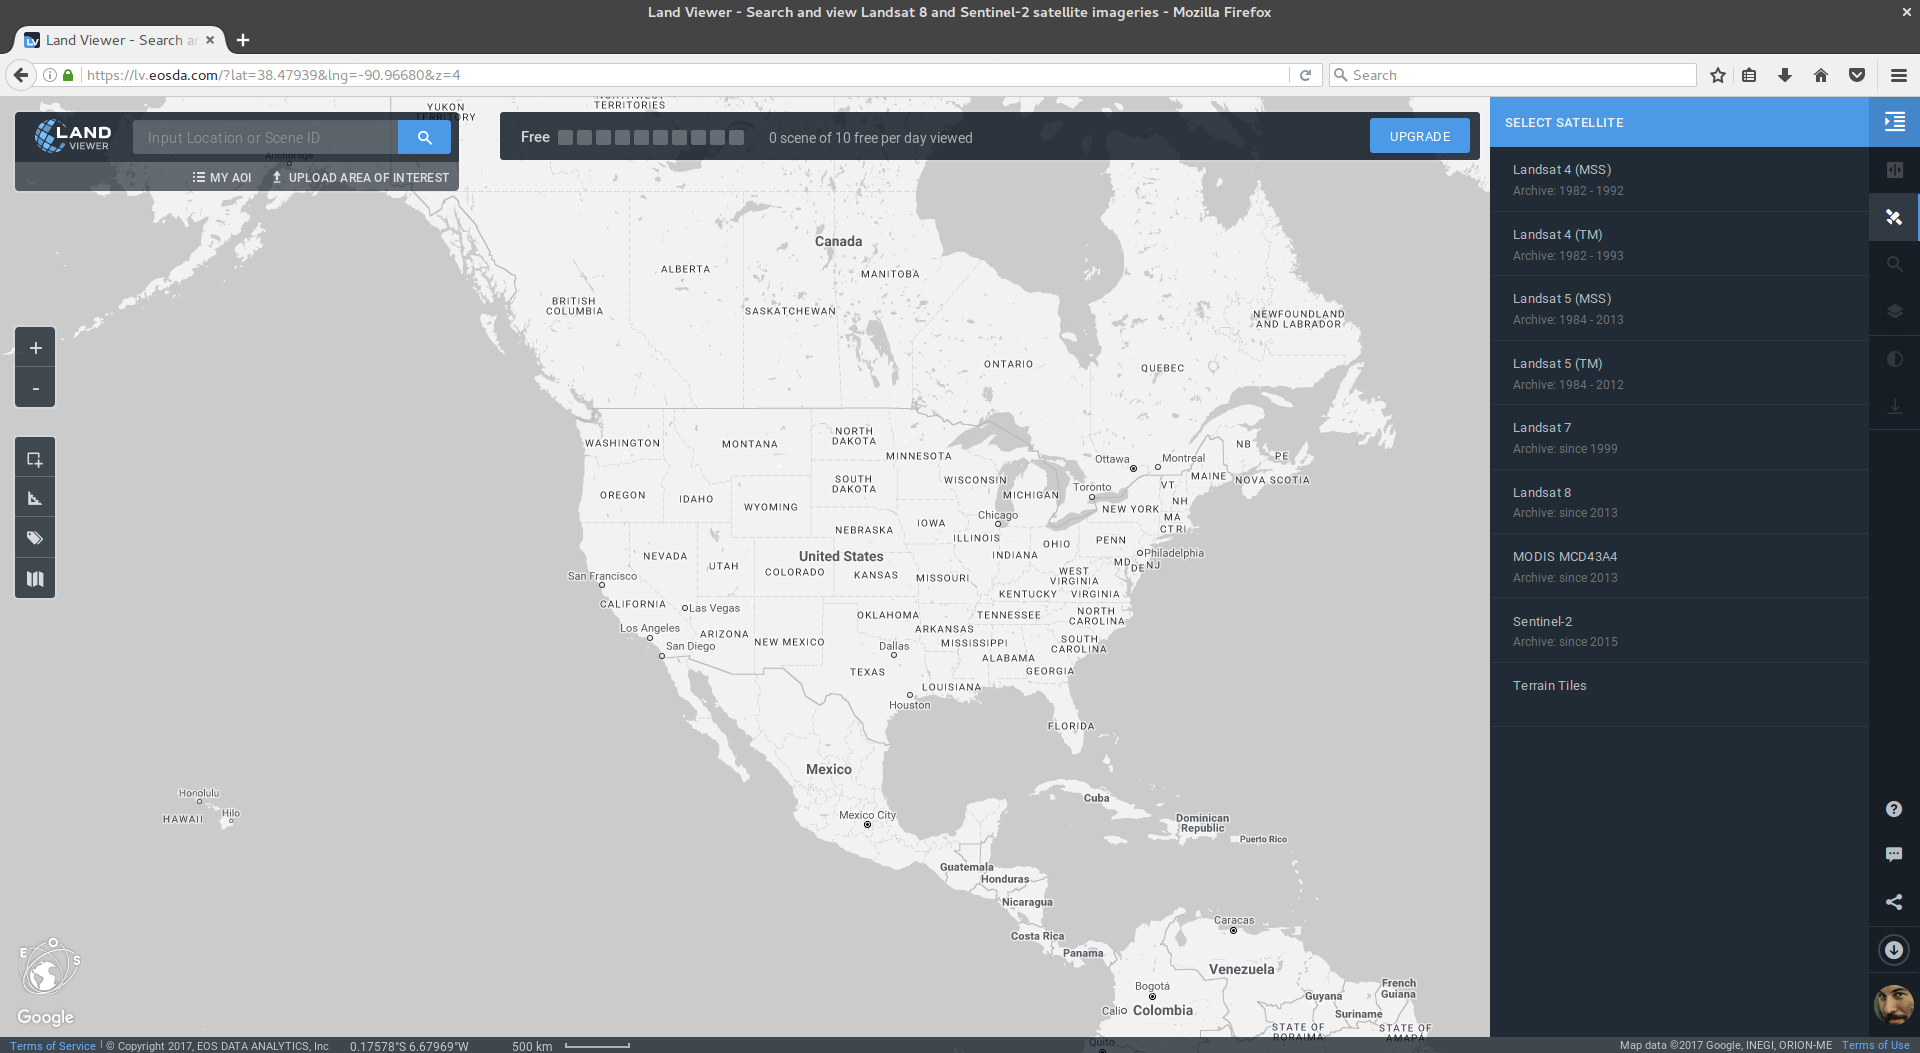
\includegraphics[width=0.85\textwidth]{fig:main.png}
    \caption{Pantalla principal del Land Viewer. Abajo a derecha de encuentra la opción de registro. A la derecha tenemos las herramietas de medición, zoom y mapas. Arriba el cuadro de busqueda. A la izquierda encontramos la selección de imágenes y productos satelitales.}
    \label{fig:main}
\end{figure}

\begin{itemize}
    \item La parte superior que nos permite buscar en el mundo.
     \begin{center}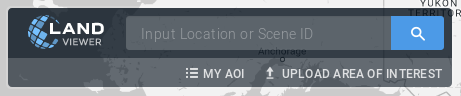
\includegraphics[scale=0.4]{in:search.png}\end{center}
    \item La parte izquierda que nos permite hacer zoom en el mapa, marcar zonas de interés, realizar mediciones y agregar distintas capas como puede ser un mapa de alturas, una imagen satelital de base o un mapa político.
     \begin{center}
\includegraphics[scale=0.4]{in:edit.png}\end{center}
    \item La parte derecha donde podemos elegir distintos productos satelitales, mostrarlos, realizar combinaciones de bandas y guardar los datos obtenidos.
     \begin{center}
\includegraphics[scale=0.4]{in:sat.png}\end{center}
\end{itemize}

Podemos ver tambien la latitud y longitud de cualquier punto posicionandonos sobre el y observando el valor en la parte inferior de la pantalla.




\section{Mediciones}

En el modo mapa, busque la ciudad de Villa Carlos Paz. Podemos utilizar la herramienta medir distancias 
\includegraphics[scale=0.2]{in:medir.png} para determinar la distancia entre Córdoba Capital y Villa Carlos Paz (Figura \ref{fig:distancia}) que es de aproximadamente $30km$ en linea recta.

\begin{figure}[!h]
    \centering
    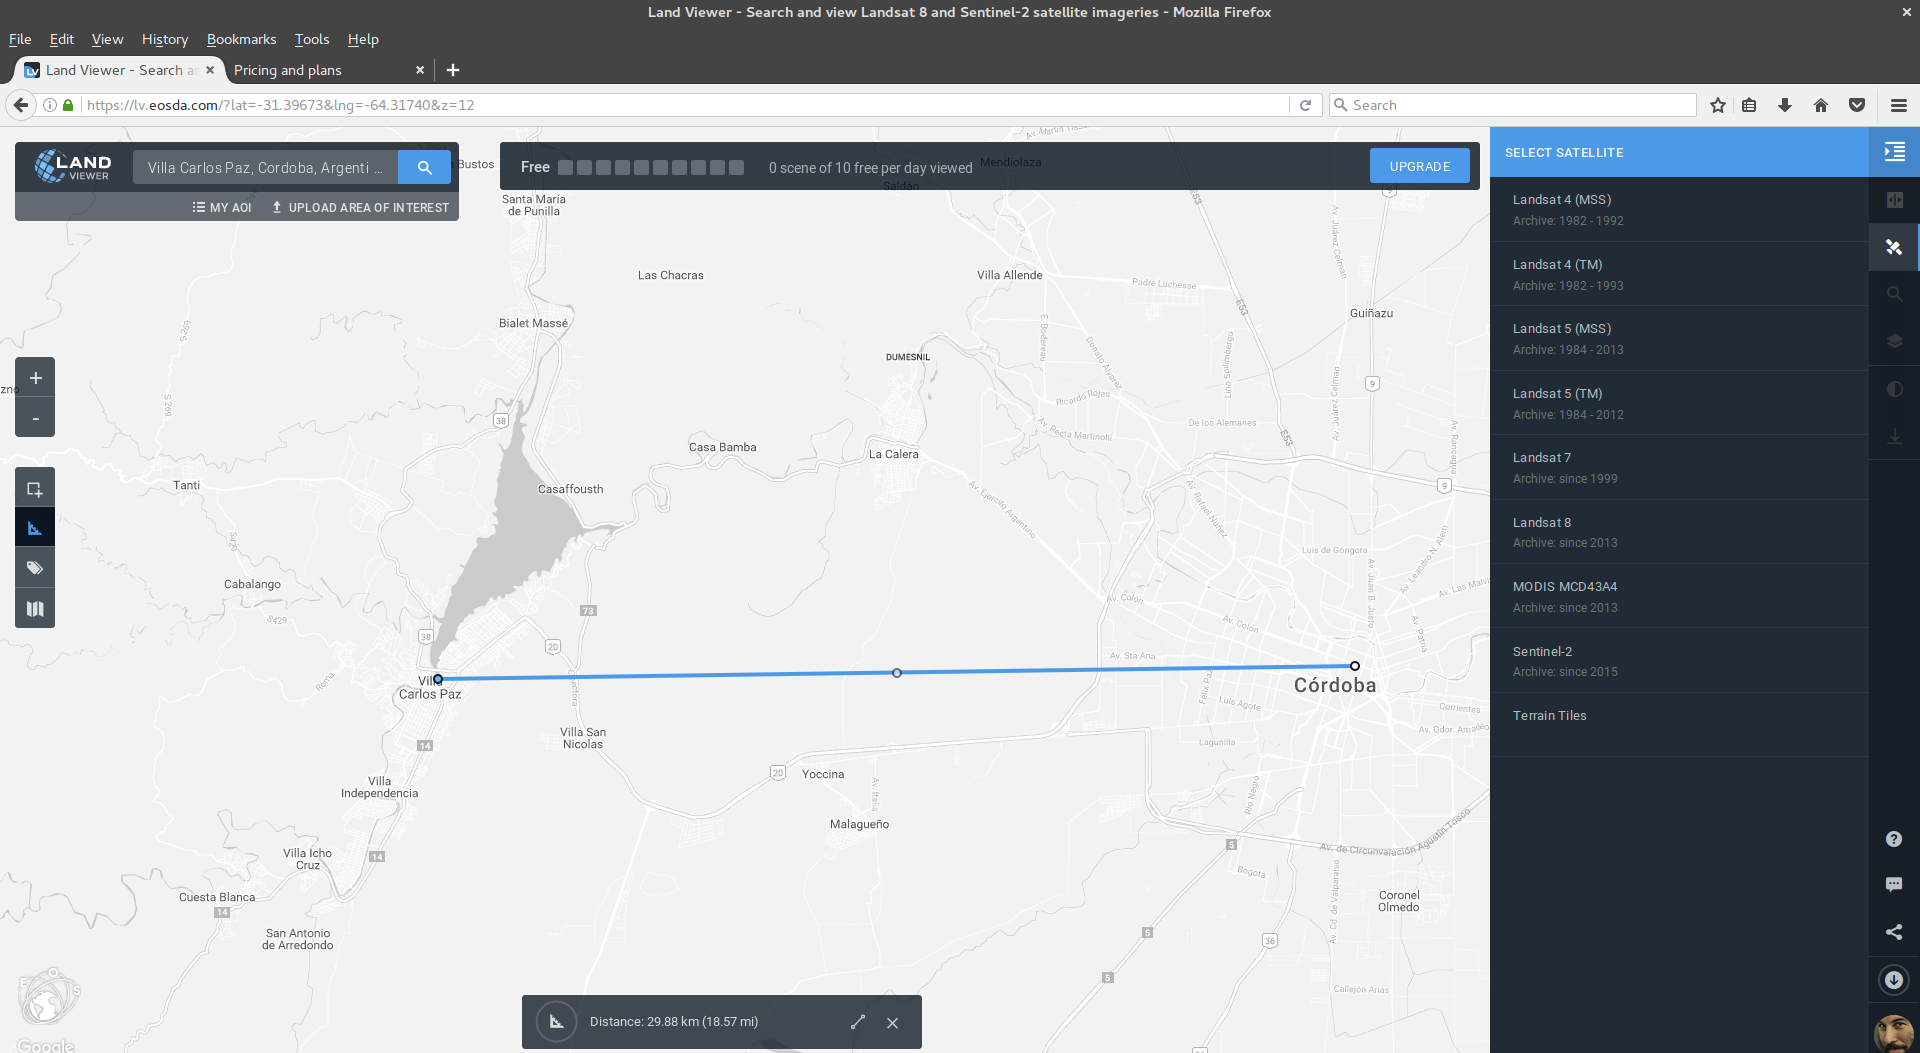
\includegraphics[width=0.85\textwidth]{fig:distancia.png}
    \caption{Medición de distancia entre la ciudad de Córdoba y Villa Carlos Paz. La distancia aparece en la parte inferior de la pantalla.}
    \label{fig:distancia}
\end{figure}

Con la misma herramienta, es posible medir áreas si uno cierra el camino obtenido sobre el primer punto.

\section{Actividades}

\begin{que}
    ¿Cual es la superficie del Lago San Roque, que se encuentra inmediatamente al norte de Villa Carlos Paz?
\end{que}
\begin{que}
    ¿Cual es el perimetro del Lago San Roque?
\end{que}
\begin{que}
    ¿Cual es la superficie del Lago de Mar Chiquita, Córdoba?
\end{que}

\begin{que}
    ¿Cuales son las coordenadas de las ciudades de Córdoba Capital, Villa Carlos Paz, Rio Cuarto y Villa Maria?
\end{que}

\begin{que}
    ¿Cual es la distancia lineal entre la ciudad de Córdoba y la ciudad de Santa Rosa en La Pampa?
\end{que}

\chapter{Resolución espacial y temporal}
Dos características fundamenteles de las imágenes satelitales son la resolución espacial y la resolución temporal.

La resolución espacial nos da una idea de que objenos podemos distinguir en el terreno. Por ejemplo, una resolución espacial de $30m$ nos permitirá distinguir una plaza de una manzana construida, pero no las casas dentro de una manzana.

A su vez la resolución temporal nos da una idea de cual es el fenomeno que varía en el tiempo más corto que podemos ver. Por ejemplo, una resolución temporal de $15$ días nos permitirá estudiar como cambia la vegetación a lo largo de las estaciones pero no como cambian las nubes a lo largo de un día.

\begin{figure}[h!]
    \centering
    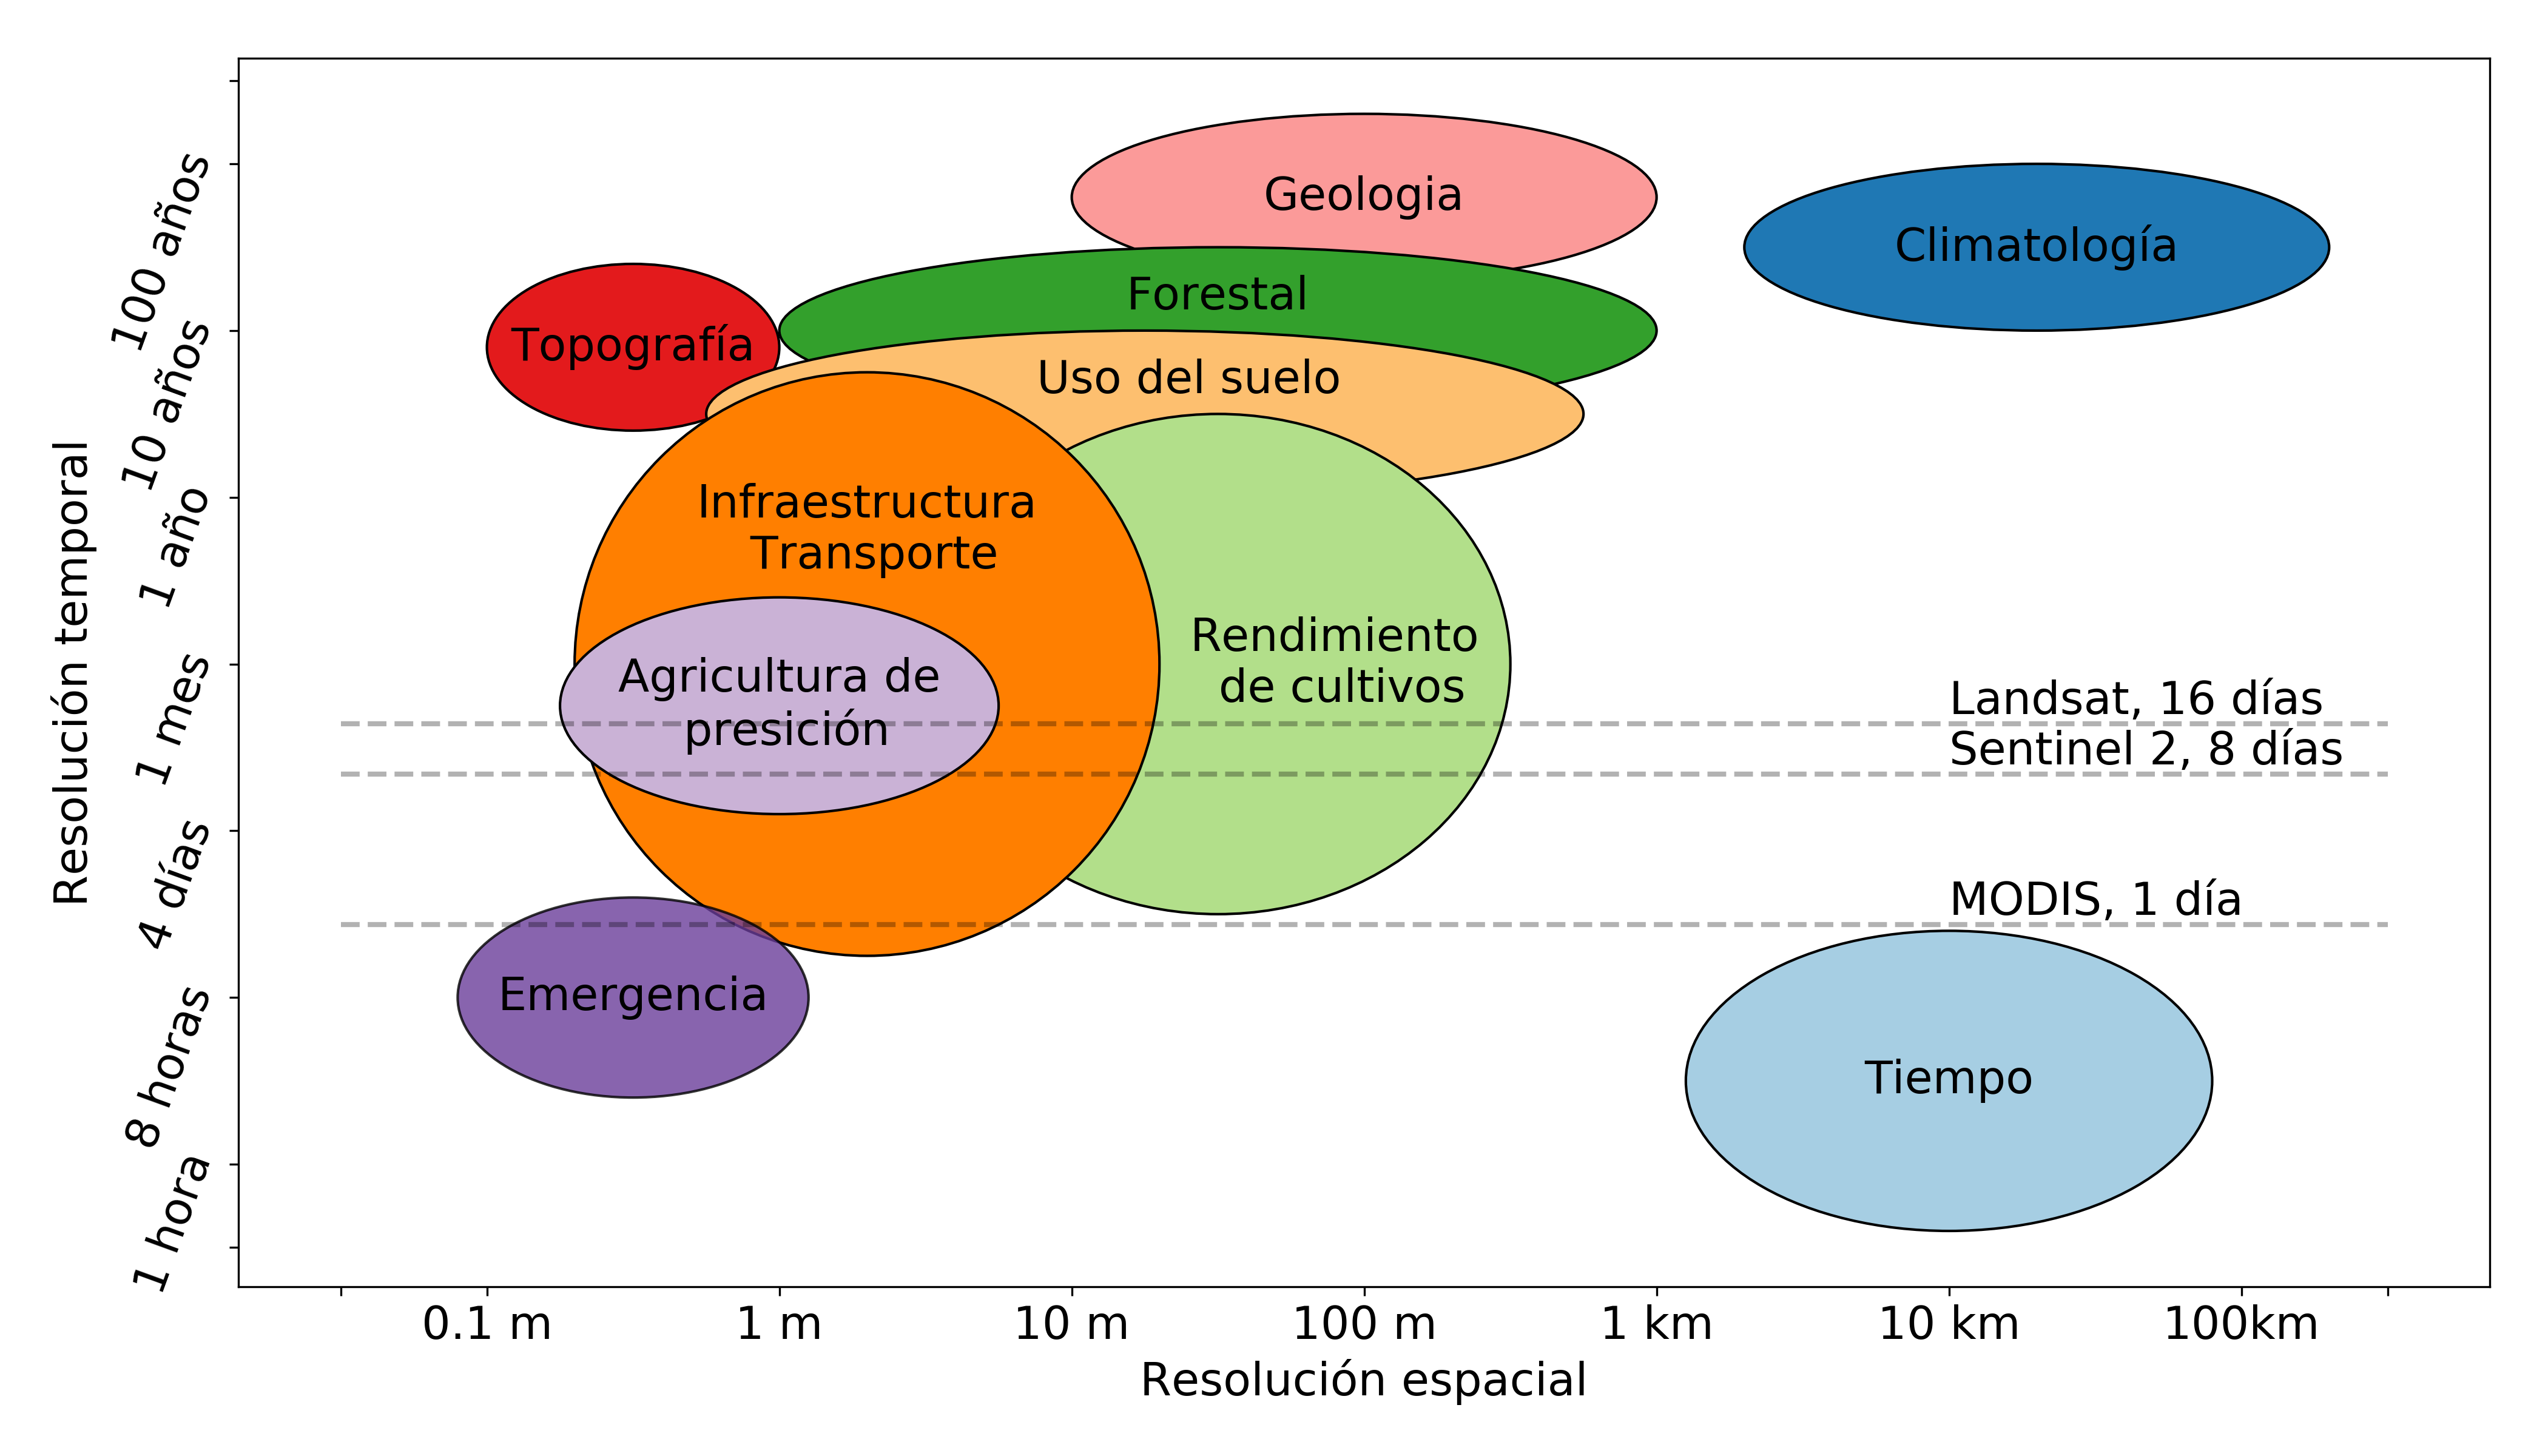
\includegraphics[width=0.85\textwidth]{fig:evst.png}
    \caption{}
    \label{fig:evst}
\end{figure}


Ambas resoluciones suelen estar relacionadas (Figura \ref{fig:evst}), de forma que al aumentar una disminuye la otra. Por ejemplo: GOES, una satélite meteorológico, tiene una muy alta revisita temporal, cercana a los 15 minutos mientras que su resolución espacial es baja, cercana a los 4km. En el otro extremo, SPOT 7 tiene una alta resolución espacial, de hasta $1.5$m, pero con una revisita temporal del orden del mes.

Es importante recordar en esta instancia que una resolución mayor o menor solo nos dice si la imagen será util para cierto estudio. No si la imagen es mejor o peor. Por ejemplo: una regla milimetrada permite medir con mucha presición, pero nunca usariamos una para medir el largo de una avenida.


\section{Imágenes satelitales}
Es posible hora incorporar imágenes satelitales a nuestro mapa. Para esto comenzamos dibujando un Área de Interes (AOI) sobre la imagen que incluya la zona entre Lago San Roque y Córdoba (Figura \ref{fig:aoi}).

\begin{figure}[h!]
    \centering
    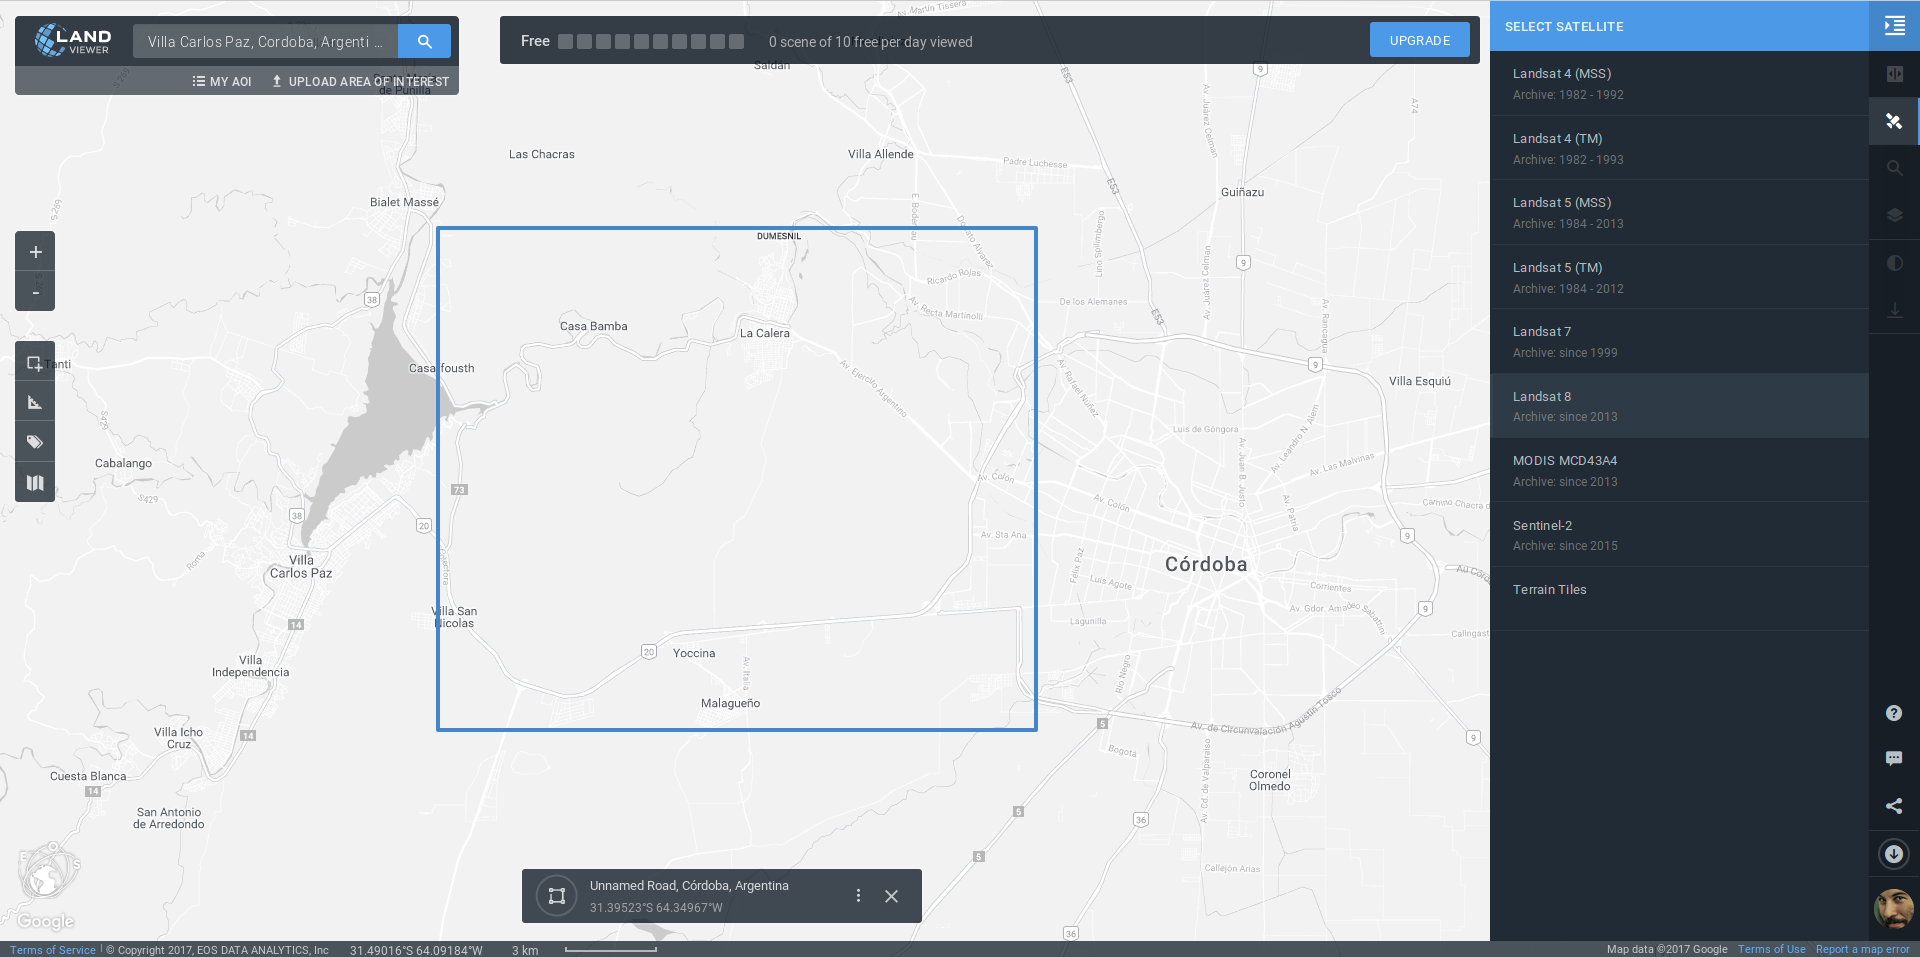
\includegraphics[width=0.85\textwidth]{fig:aoi.png}
    \caption{Gráfico de un área de interes (AOI) para seleccionar la zona en la que se seleccionaran las imagenes.}
    \label{fig:aoi}
\end{figure}

Elija ahora el satélite Landsat 8 y observe que pareceran distintas escenas a la derecha. Por defecto Land Viewer muestra solo las escenas con cobertura nubosa de hasta un 60\% y de los últimos 3 meses. Es posible cambiar esto haciendo click en la parte superior del Scene Search.  Ponga la cobertura nubosa hasta el 100\%.

\begin{center}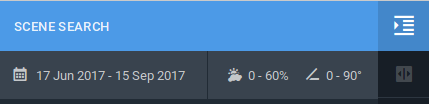
\includegraphics[scale=0.4]{in:nubes.png}\end{center}

Seleccione la imagen del 2 de septiembre de 2017 (Figura \ref{fig:scene}) y observe que esta aparecerá en la pantalla. Puede ahora moverse como hacía antes y realizar mediciones.

\begin{figure}[h!]
\centering
\begin{minipage}{.425\linewidth}
  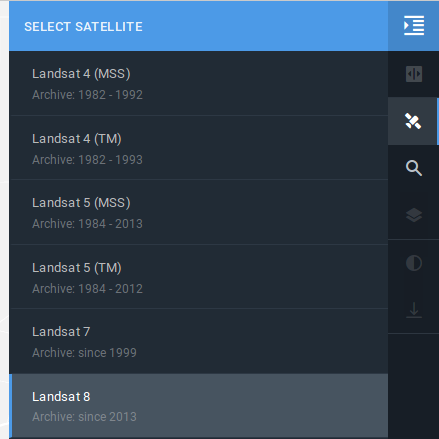
\includegraphics[width=\linewidth]{fig:sat.png}
\end{minipage}
\hspace{.05\linewidth}
\begin{minipage}{.425\linewidth}
  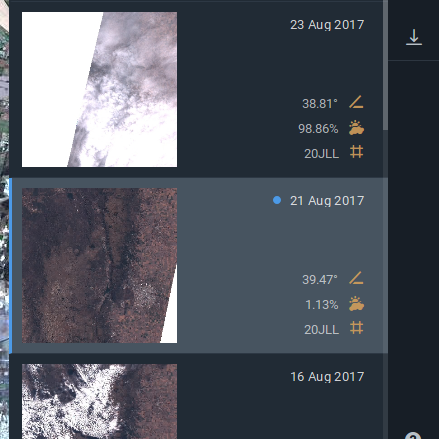
\includegraphics[width=\linewidth]{fig:imagen1.png}
\end{minipage}
\caption{Selección de satélite e imágenes en Land Viewer.}
\label{fig:scene}
\end{figure}

La imagen elegida pertenece al sensor OLI del satelite Landsat 8. Tiene una resolución espacial de $30m$ por lo cual podremos distinguir manzanas, parques y objetos más grandes, pero no más chicos.

Seleccione ahora el producto MODIS MCD43A4. Verá en este caso que la lista de imágenes es mucho más densa teniendo una imagen por día. Seleccione la imagen correspondiente al 27 de agosto de 2017.

Observe que ahora no es posible distinguir las manzanas de la ciudad de Córdoba como hacía con la imagen anterior. En este caso la imagen elegida pertenece al producto \emph{MCD43A4} generado a partir del sensor MODIS de los satélites AQUA y TERRA. En este caso la resolución espacial oscila entre los 250m y los 1000m según como mostremos la imagen.

\section{Comparación entre fechas}
Comparemos ahora dos imágenes antes y después del incendio. Para esto seleccione el satélite Sentinel 2 y elija la imagen del 21 de agosto de 2017. Haga luego click en \emph{Comparison slider} 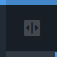
\includegraphics[scale=0.2]{in:LR.png}, cambie la fecha al año 2016 y seleccione la imagen del 23 de agosto de 2016.

Es posible elegir si la imagen se posiciona a la izquierda o la derecha eligiendolo en el botón L/R.

\begin{center}
\includegraphics[scale=0.4]{in:LorR.png}\end{center}

Puede mover ahora el slider a la izquierda y la derecha para comparar las imágenes del 2016 y 2017 (Figura \ref{fig:slider}). Elegimos comparar con el año anterior para que las imágenes correspondan a fechas similares.

\begin{figure}[h!]
    \centering
    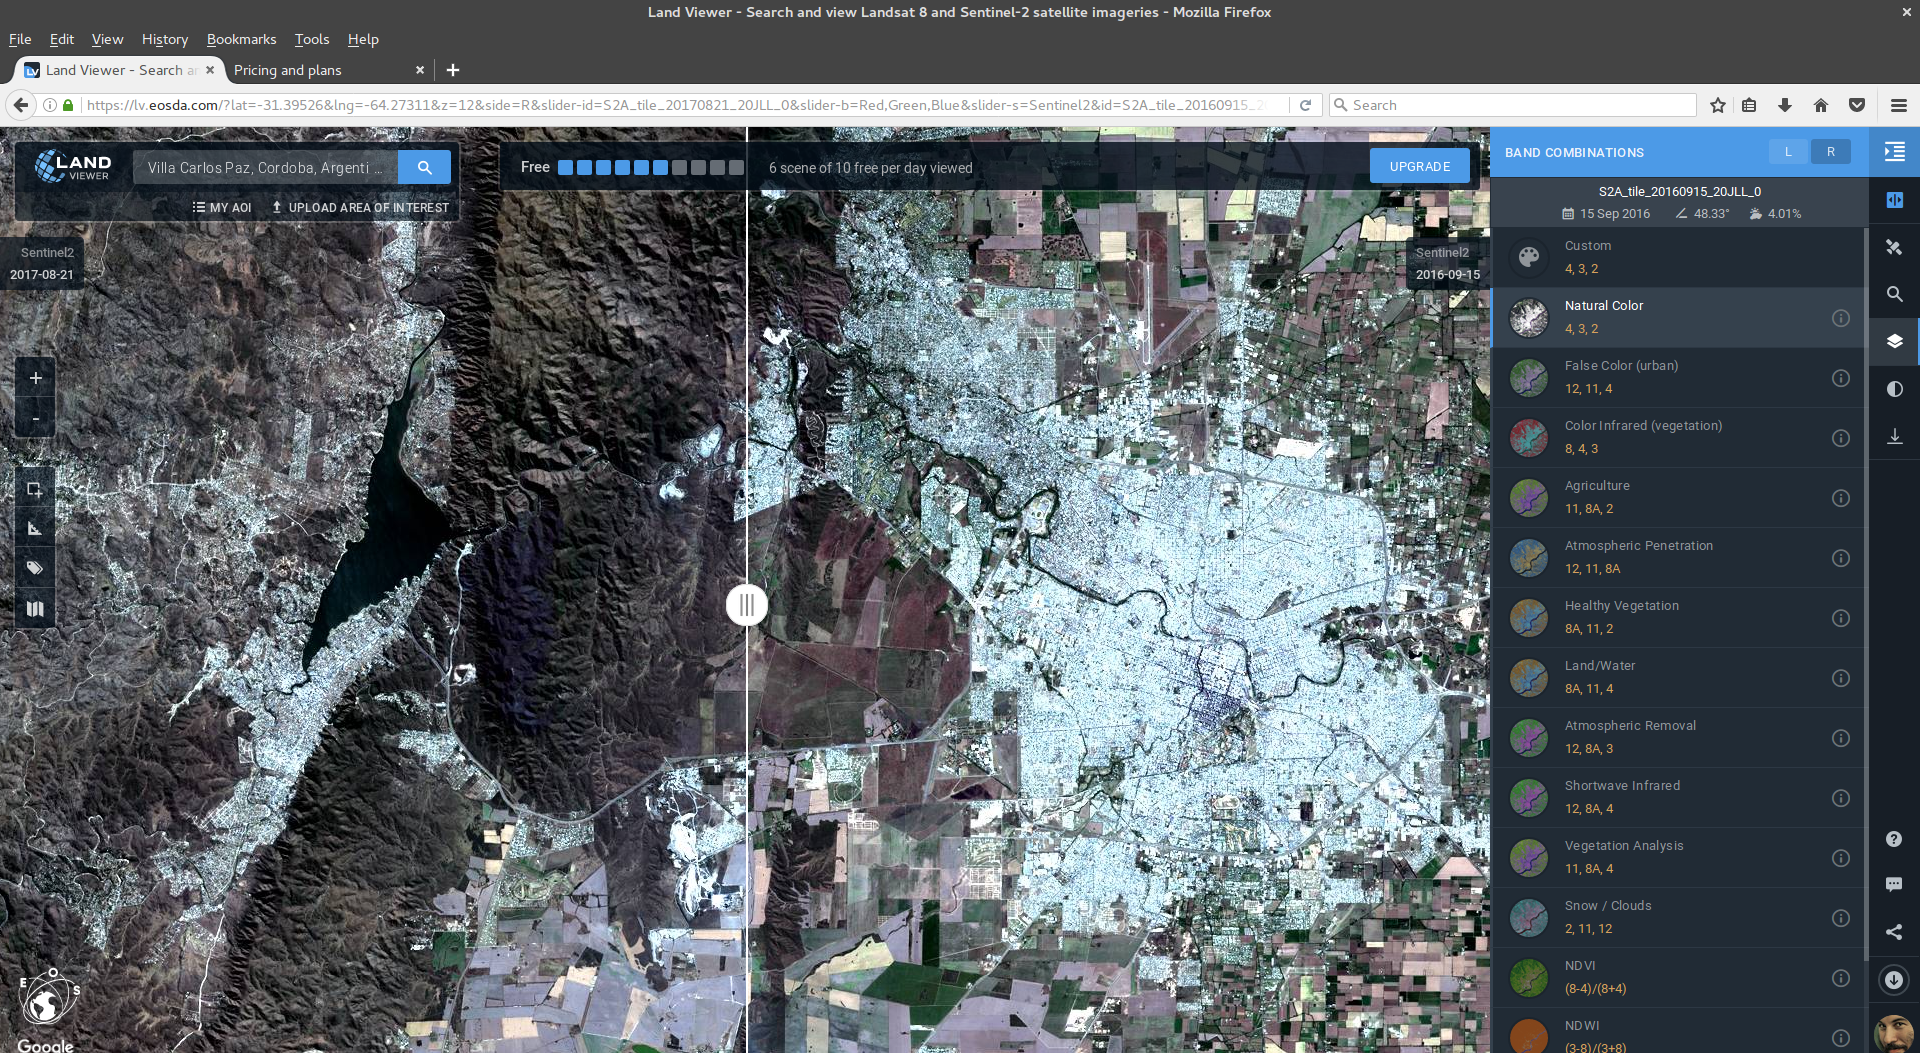
\includegraphics[width=0.85\textwidth]{fig:slider.png}
    \caption{Dos imágenes con la pantalla dividida. En el medio aparece el slider que permite cambiar entre las dos zonas.}
    \label{fig:slider}
\end{figure}

\section{Actividades}
\begin{que}
    ¿Cada cuantos días hay una nueva imagen Landsat 8?
\end{que}
\begin{que}
    ¿Cada cuantos días hay una nueva imagen MODIS?
\end{que}
\begin{que}
    ¿Es posible distinguir las manzanas de la Ciudad de Cordoba en la imagen Landsat 8?
\end{que}
\begin{que}
    ¿Hay incendios en la zona durante el año 2016?
\end{que}
\begin{que}
    ¿Que superficie tiene el área incendiada dentro de la imagen?
\end{que}

\chapter{Combinaciones espectrales}
Si llego hasta acá, notará que en la combinacion de colores que estamos observando la imagen, a pesar de ser intuitiva, no permite distinguir claramente las zonas incenciadas

Para mejorar la detección del incendio es necesario entender que un satélite, como cualquier sensor, puede ser configurado para medir distintas coberturas. En este caso, el satélite mide la cantidad de luz\footnote{Conocida como radiancia en teledetección.} que proviene de la superficie terrestre como hacen nuestros ojos. Sin embargo, a diferencia de nuestros ojos es posibles cambiar la zona del espectro electromagnético donde medimos y como la mostramos.

\begin{figure}[h!]
    \centering
    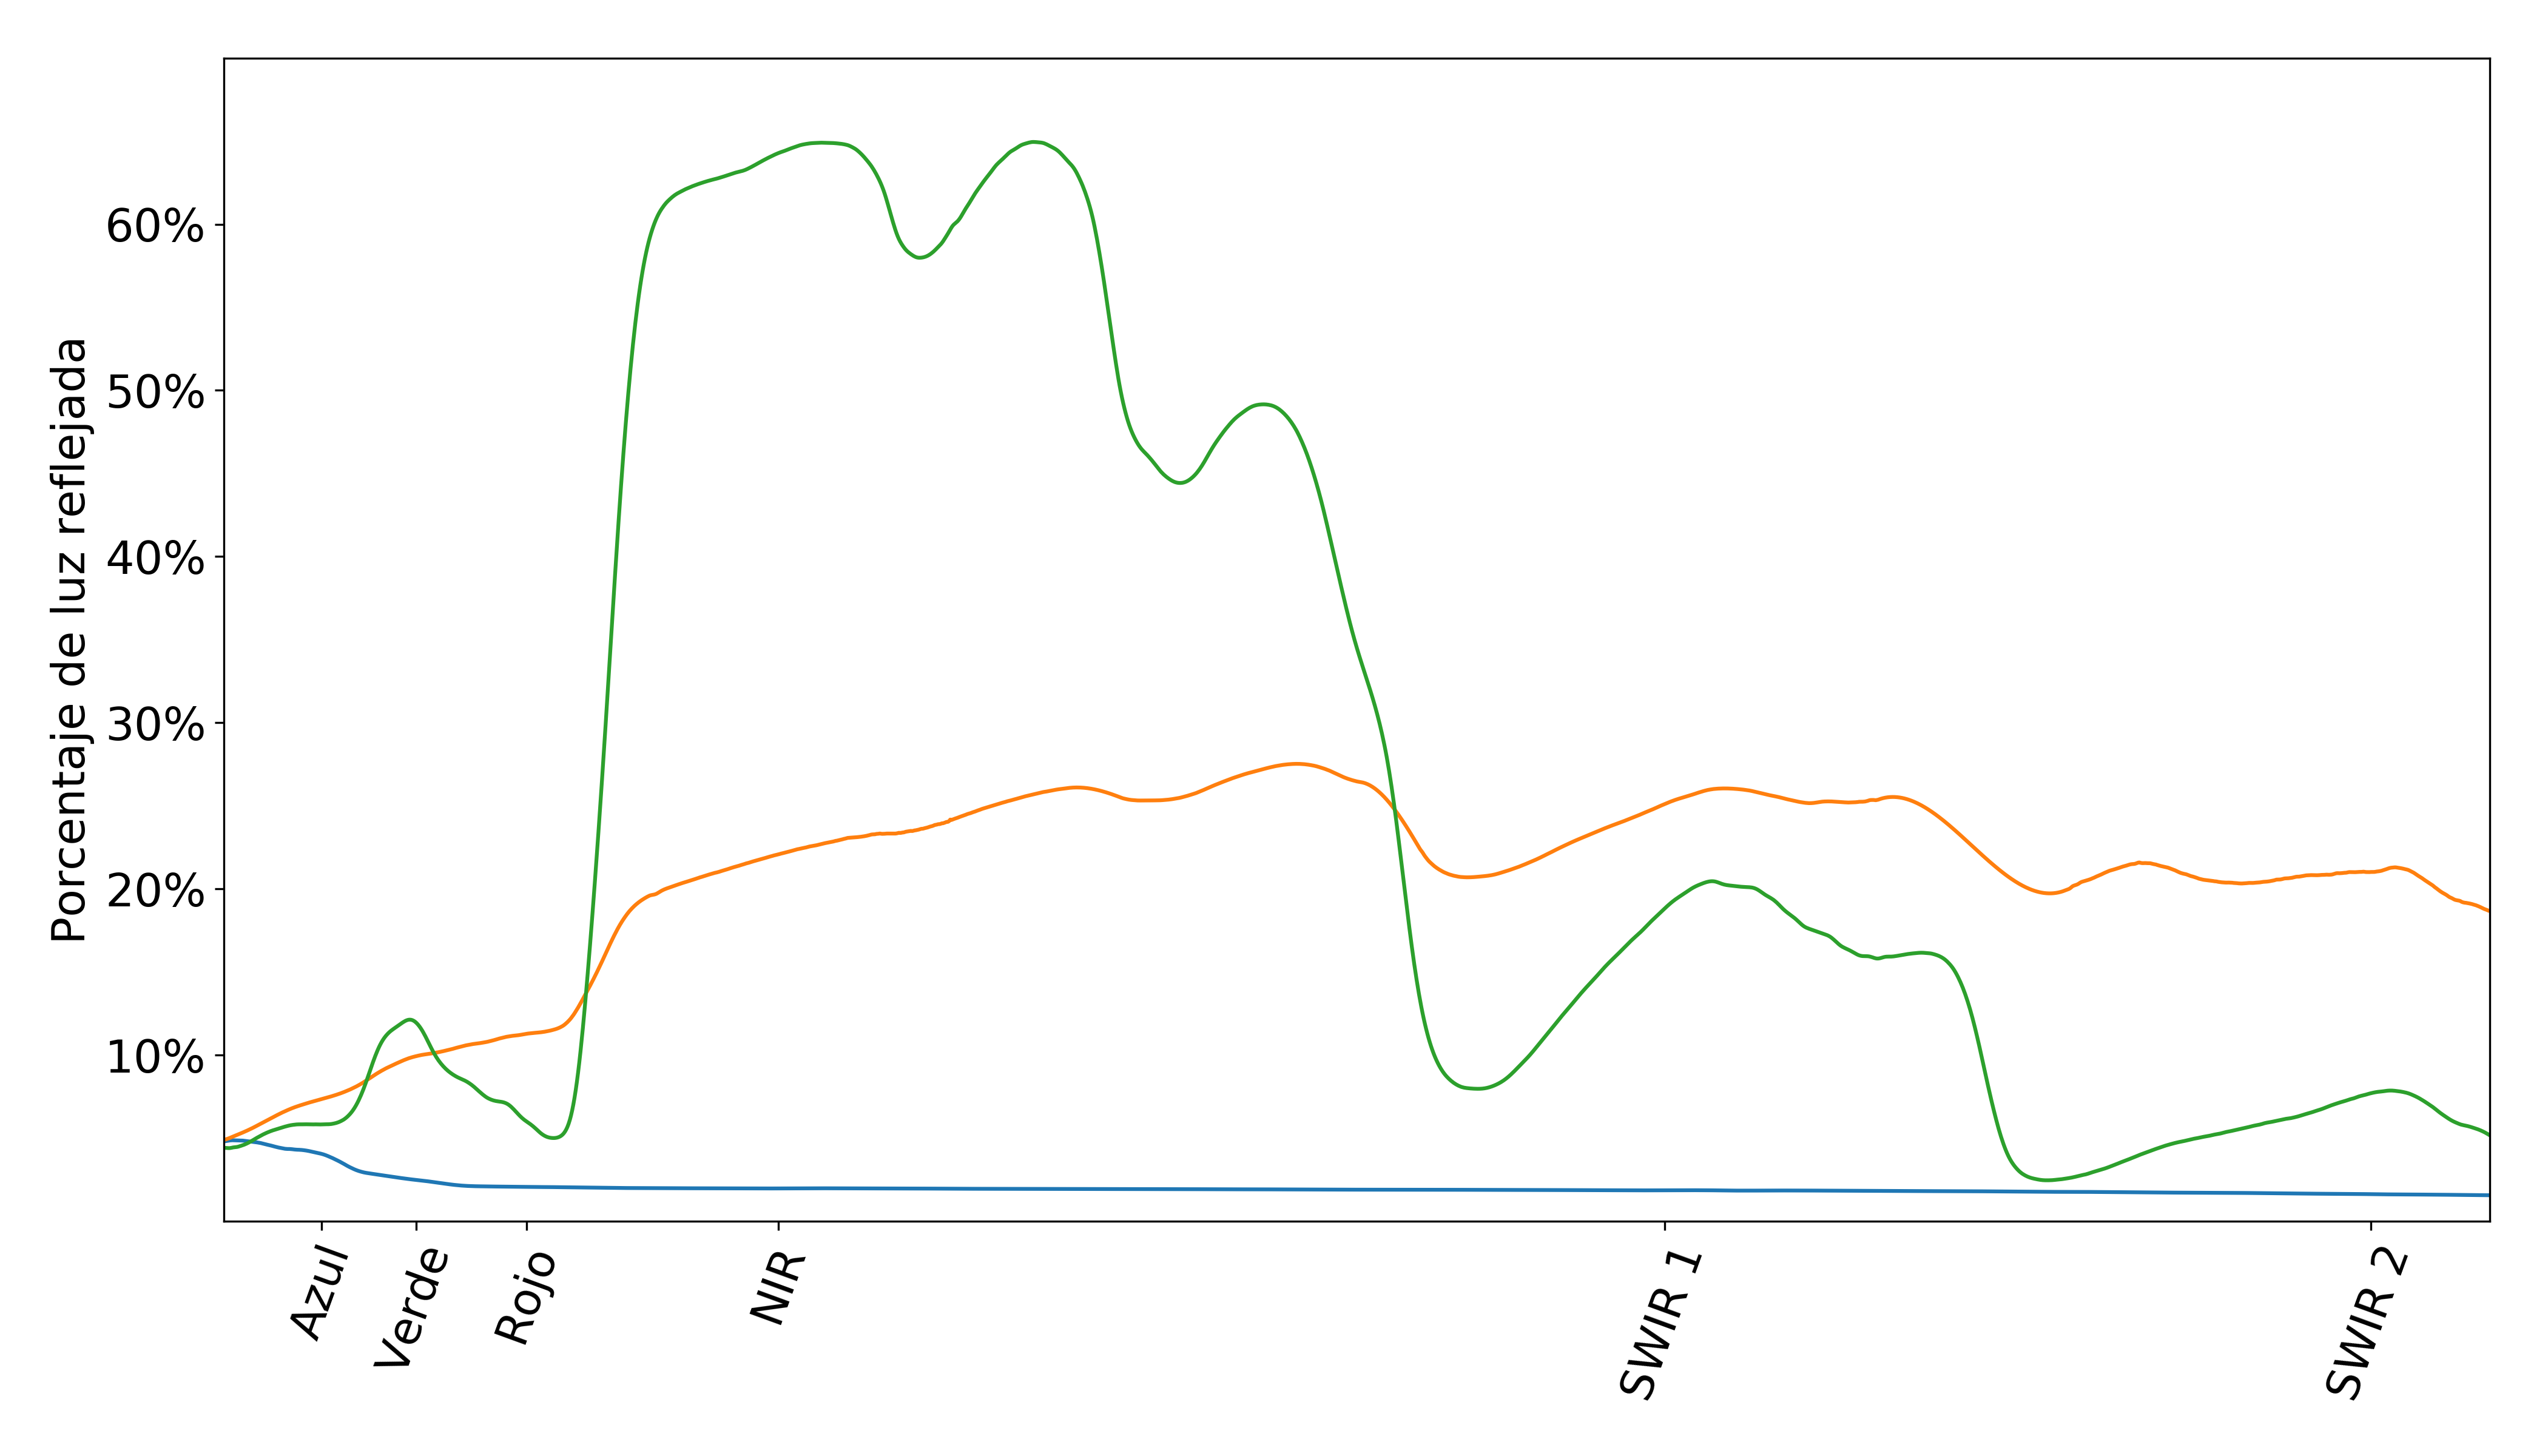
\includegraphics[width=0.85\textwidth]{fig:spec.png}
    \caption{Firmas espectrales para el agua, suelo y vegetación.}
    \label{fig:spec}
\end{figure}

Esto es importante porque cada zona del espectro electromagnético aporta distinta información sobre las coberturas del suelo. Si miramos cuanta luz nos llega para coberturas de vegetación, suelo sin cobertura vegetal y cuerpos de agua, observamos que cada una de ellas se comporta de distinta manera como función de la longitud de onda (Figura \ref{fig:spec}).

\section{Combinaciones RGB}

Para aprovechar esto, realizamos las que se llaman combinaciones RGB. Mostrando de color rojo, verde y azul distinta información.

Para cambiarlas en Land Viewer, haga click en BAND COMBINATIONS (Figura \ref{fig:bandas}).

\begin{figure}[h!]
    \centering
    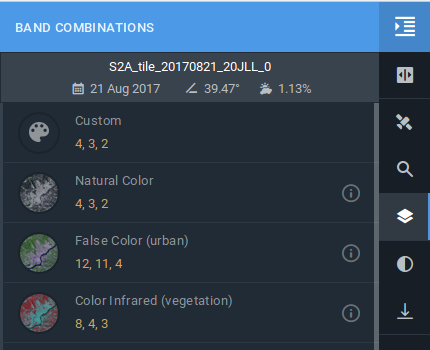
\includegraphics[width=0.4\textwidth]{fig:bandas.png}
    \caption{Ventana para elegir distintas combinaciones de bandas. Es posible tanto elegir una pre-armada o configurar una a mano.}
    \label{fig:bandas}
\end{figure}

Distintas combinaciones de bandas permiten mostrar distinta información:

\begin{itemize}
    \item Color real (\emph{Natural color - rojo,verde,azul}): Muestra la imagen de forma similar a como la verían nuestros ojos. Las bandas del espectro visible se asignan para que coincidan con  las del ojo. La vegetación se ve verde. Los suelos y distintos tonos de marrón. Las ciudades en blanco. Los cuerpos de agua se muestran en colores oscuros.
    \begin{center}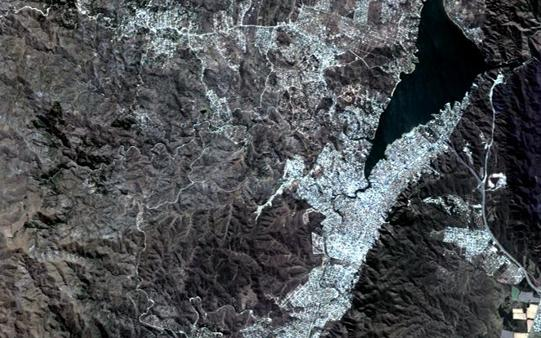
\includegraphics[scale=0.3]{4-3-2.jpeg}\end{center}
    \item Falso color (\emph{False color (urban) - SWIR2,SWIR1,Rojo}): Provee una imagen similar a como la interpretarían nuestros ojos pero eliminando parte de la incidencia de la atmósfera. La vegetación aparece en verde. Las zonas urbanas en blanco y ciam. Los suelos en una variedad de colores. Las zonas con agua aparecen en azul o negro.
    \begin{center}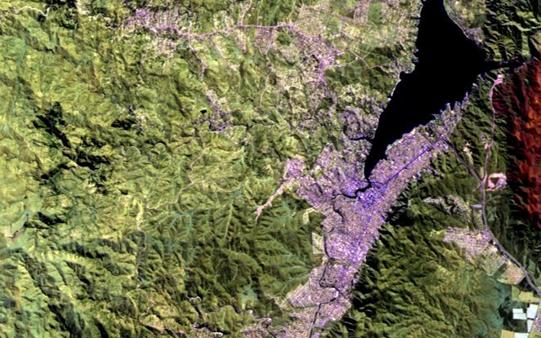
\includegraphics[scale=0.3]{12-11-4.jpeg}\end{center}
    \item Infrarrojo color (\emph{Color infrared (vegetation) - NIR, Rojo, Verde}): La combinación de color standar para separar vegetación de otras coberturas. La vegetación suele verse en color rojo brillante. Las ciudades y suelos sin cobertura se ven en tonos de cyan. Las zonas con agua se ven en negro.
    \begin{center}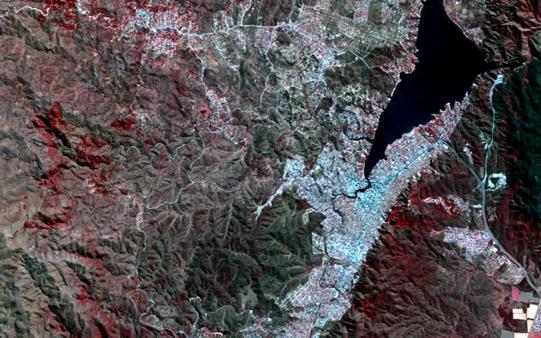
\includegraphics[scale=0.3]{8-4-3.jpeg}\end{center}
    \item Falso color (\emph{Land/water - NIR, SWIR1, Rojo}): Combinación de bandas útil para separar agua de vegetación y obtener características sobre esta última. La vegetación se verá en tonos de naranja, dependiendo de su contenido de humedad. Las zonas con agua en azul. Las ciudades y suelos desnudos en blanco y verde.
    \begin{center}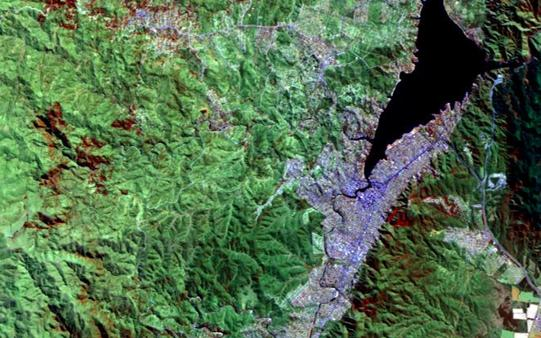
\includegraphics[scale=0.3]{8-11-4.jpeg}\end{center}
\end{itemize}

En nuestro caso particular, la combinación de bandas que mejor separa las zonas incenciadas de las no incendiadas es la \emph{Short wave infrared}. Esta combinación muestra en rojo las zonas que se incendiaron recientemente y en verde las zonas con vegetación. Eligala en el Land Viewer y compare la imagen antes y después del incendio (Figura \ref{fig:incendio}).

\begin{figure}[h!]
    \centering
    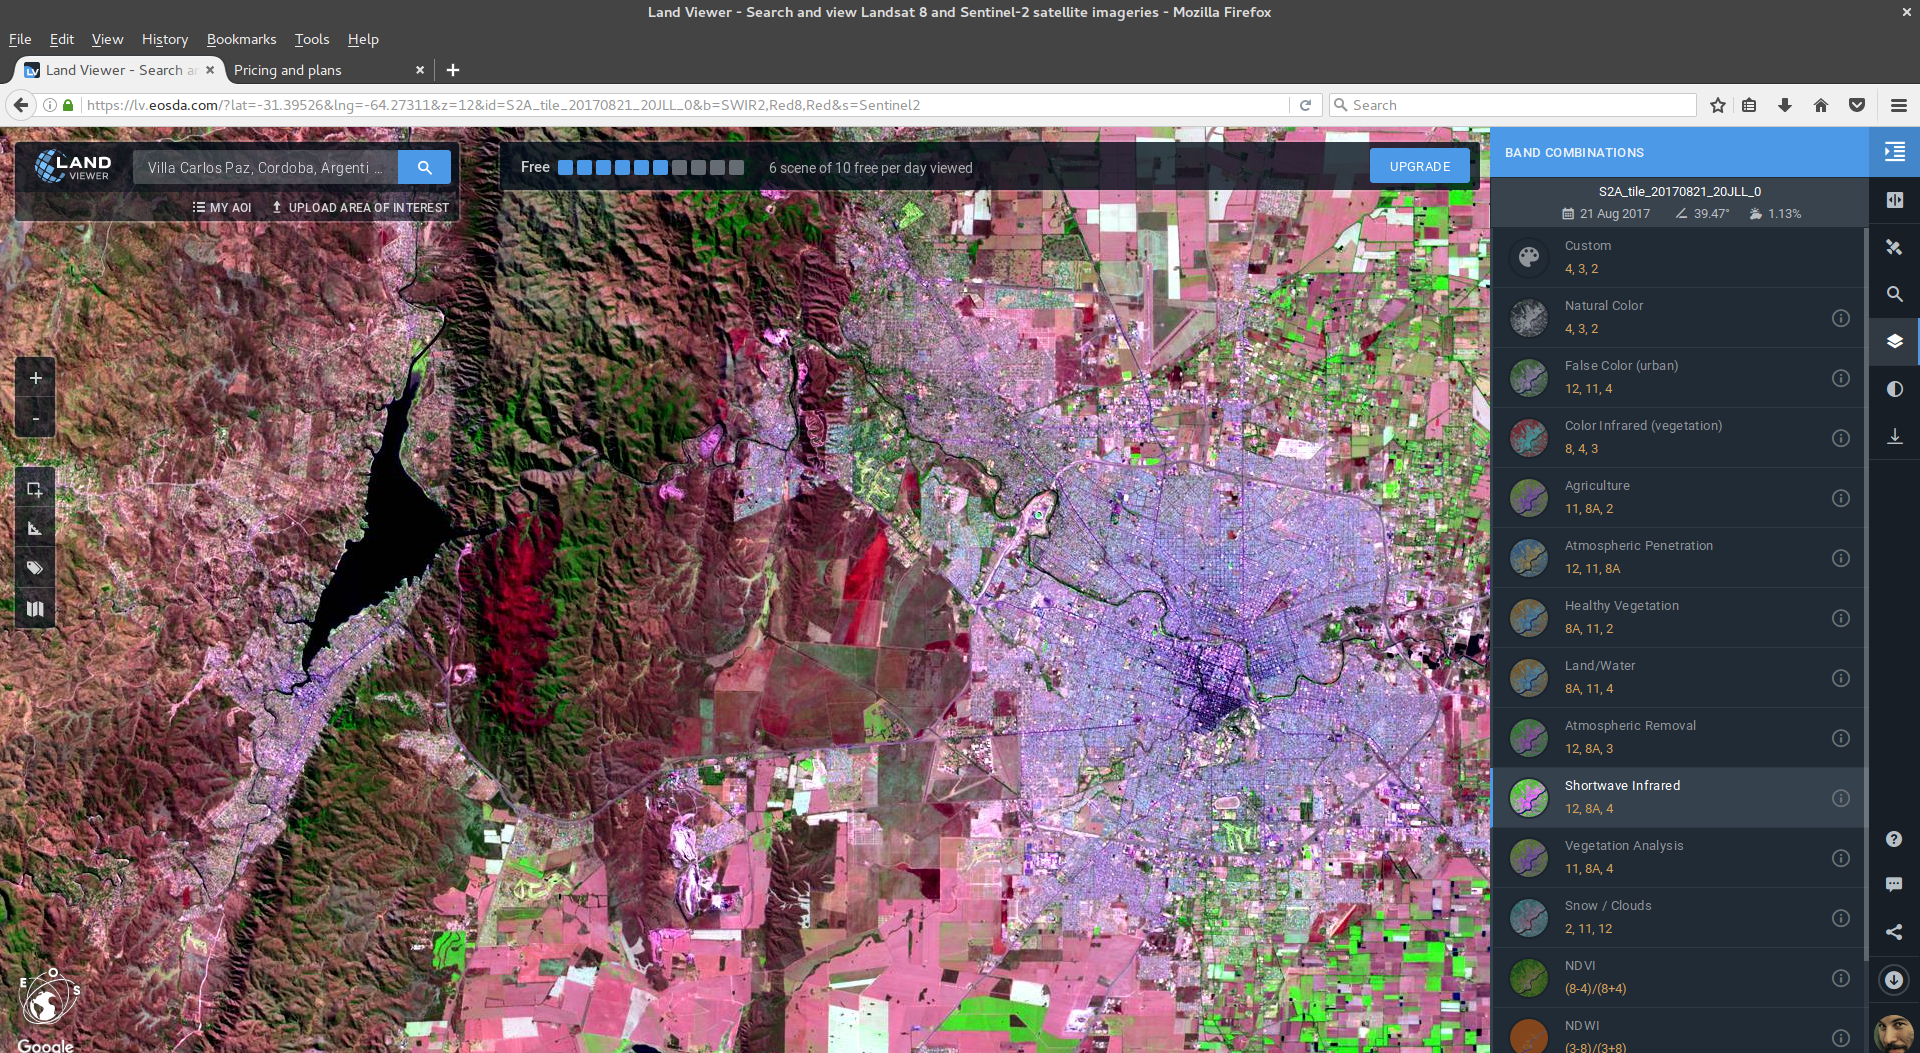
\includegraphics[width=0.85\textwidth]{fig:incendio.png}
    \caption{Imagen en la combinación de colores que mejor resalta al incendio. La vegetación se ve en colores verde brillante, el incendio en rojo, el agua negro y la ciudad en violeta.}
    \label{fig:incendio}
\end{figure}

Puede descargar la imagen generada haciendo click en ESCENE DOWNLOAD, eligiendo la opción de \emph{Crop by extent} y luego haciendo click en Download.

\section{Actividades}

\begin{que}
    ¿Cual es la superficie incendiada al oeste del Lago San Roque?
\end{que}

\begin{que}
    ¿En que color se la zona incendiada en cada una de las combinaciones de bandas descriptas arriba?
\end{que}

\begin{que}
    ¿Que combinación de bandas le permite distinguir más detalles en el Lago San Roque?
\end{que}

\begin{que}
    ¿Que combinación de bandas le permite distinguir mejor vegetación dentro de la ciudad de Córdoba?
\end{que}

\begin{que}
    ¿Cuanto creció la superficie incendiada entre el 21 de agosto y el 17 de septiembre de 2017 al este de Villa Carlos Paz?
\end{que}

\begin{que}
    Descargue un mapa de la zona donde se vea la superficie incendiada al 21 de agosto de 2017 en las cercanias de Villa Carlos Paz.
\end{que}

\chapter{Cierre}

Vimos en este taller actividad como utilizar las herramientas del LandView junto con nuestro conocimiento en teledetección para interpretar distintas coberturas.

Aprendimos que hay 3 características fundamentales de un conjunto satélite/sensor a la hora de usar productos geoespaciales

\begin{itemize}
    \item Resolución espacial: que tan bien puedo distinguir un objeto en el terreno.
    \item Resolución temporal: cada cuanto vuelvo a tener una imagen de la misma zona.
    \item Resolución espectral: cuantas zonas del espectro puedo distinguir.
\end{itemize}

Este es el puntapié inicial al trabajo en teledetección donde la interpretación visual se combina con el procesamiento digital para extraer información sobre la tierra. Los invitamos a que sigan de aquí en adelante.


\end{document}
